\section{Musical Preliminaries}
\label{sec:music}

\paragraph{Pitches}
In music, a \emph{pitch} is a value denoting how high or low a sound is.
Pitches can be represented either as an absolute value or as a relative
value paired with the octave the sound belongs to.
In our implementation, the two representations of pitches are defined
as the \texttt{Pitch} and \texttt{PitchOctave} datatypes, respectively,
accompanied by a proof that converting back and forth between them
is an identity.

% \begin{alltt}
% data Pitch : Set where
%   pitch : \(\mathbb{N}\) \(\rightarrow\) Pitch

% data Octave : Set where
%   octave : \(\mathbb{N}\) \(\rightarrow\) Octave

% PitchOctave : Set
% PitchOctave = Fin 12 \(\times\) Octave
% \end{alltt}

\paragraph{Duration}
\emph{Duration} denotes a certain unit of time during which a sound
or silence lasts.
The unit is unspecified at the composition time; it is instantiated to
a concrete value when the music is played at a specific tempo.

% \begin{alltt}
% data Duration : Set where
%   duration : \(\mathbb{N}\) \(\rightarrow\) Duration
% \end{alltt}

\paragraph{Notes}
Combining pitches and duration gives us \emph{notes}.
In our implementation, we represent notes as a datatype \texttt{Note}
with two constructors: \texttt{tone} for notes with sound and
\texttt{rest} for those without.

% \begin{alltt}
% data Note : Set where
%   tone : Duration \(\rightarrow\) Pitch \(\rightarrow\) Note
%   rest : Duration         \(\rightarrow\) Note
% \end{alltt}

\paragraph{Intervals}

\emph{Intervals} are yet another key concept in music.
An interval denotes the difference in pitch between two notes.
There are 13 kinds of interval within an octave, and these intervals
may be classified from several different perspectives: (i) major or minor;
(ii) consonant or dissonant; and (iii) perfect or imperfect.
As a convention, we refer to \texttt{min2} and \texttt{maj2}  uniformly
as ``2nd'', and similarly for other intervals.
We also call \texttt{per1} the \emph{unison} in the rest of this section.

\begin{figure}[h]
  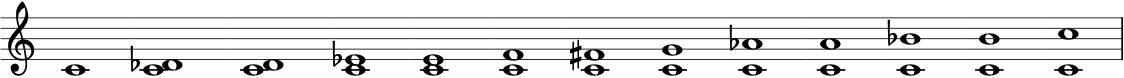
\includegraphics[width=12cm]{fig/interval.png} \\
  \begin{flushleft}
    \begin{footnotesize}
      \hspace{1.45cm} \texttt{per1 \hspace{0.5mm} min2  \hspace{2.5mm}
        maj2 \hspace{1.2mm} min3 \hspace{0.5mm} maj3 \ per4
        \hspace{1mm}aug4
        \hspace{0.5mm}  per5\hspace{1.2mm}  min6\hspace{1.6mm} maj6
        \hspace{1.6mm}min7\hspace{1.2mm} maj7\hspace{1.2mm} per8} \\
      consonant? \hspace{1.5mm} yes \hspace{4mm} no \hspace{7mm}  no
      \hspace{4.5mm} yes \hspace{3.8mm}  yes \hspace{3.5mm} no \hspace{3.5mm}
      no \hspace{4mm} yes \hspace{4mm} yes \hspace{3.2mm} yes
      \hspace{3.7mm} no \hspace{4mm} no \hspace{3.8mm} yes
    \end{footnotesize}
  \end{flushleft}
\end{figure}